\documentclass[journal]{IEEEtran}

\usepackage{amsmath}
\usepackage{amssymb}
\usepackage{pgfplots}
\usepackage{comment}
\usepackage{tikz}
\usetikzlibrary{spy}
\pgfplotsset{compat=newest}
\usepackage{float}
\usepackage{hyperref}

\begin{document}

\title{Investigations About “Singularity”:\\ Mathematical Foundation and Mechanical Interpretation}
\author{Max Erdelmeier}
\markboth{Seminar: Embedded Systems and Robotics 2023/2024, RRLAB, Rheinland-Pf\"{a}lzische Technische Universit\"{a}t Kaiserslautern-Landau}{Second Header}

\maketitle


\begin{abstract}
% change sentence structure
Singularities pose significant challenges in both robotics and general mechanical simulation.
This paper presents the mathematical foundations of singularities and
establishes a crucial link between theoretical concepts and real-world engineering applications.
Starting with the mathematical aspects, we explore the definitions of singular functions and Jacobian matrices.
Continuing with an examination of classical physics, we investigate the displacement of points on a loaded halfplane.
By comparing simulated results with real-world outcomes,
we gain an intuitive understanding of how singularities manifest in practical scenarios.
Turning our focus to robotics, we explore the kinematic foundations of robot path planning and the issues that arise from it.
Subsequently, we delve into the complexities of a simple arm robot,
which can exhibit multiple states leading to the same position of the work point.
The analysis of the simple arm robot involves exploring Jacobian matrices to detect singularities.
This multifaceted approach provides insights into the diverse manifestations of singularities in robotic systems.
By seamlessly integrating mathematical foundations with real-world examples,
this paper helps gain a more profound understanding of singularities and their implications in both theoretical and practical contexts.
\end{abstract}


\section{Introduction}
\IEEEPARstart{I}n the realms of robotics, mechanical engineering, and mathematical analysis, the term ``singularity'' holds a pivotal and multifaceted significance.
Singularities represent critical junctures where conventional rules and models encounter challenges,
prompting a closer examination of their implications on both theoretical frameworks and practical applications.

The term itself spans diverse fields, each offering unique perspectives on the concept.
In the context of robotics, singularities manifest as pivotal points where robotic systems face inherent limitations,
leading to unexpected behaviors and constrained motion.
These phenomena present intricate challenges that demand a comprehensive understanding of the underlying mathematical foundations.

Beyond the domain of robotics, singularities find their roots in geometry, complex and real analysis.
This paper delves into the mathematical intricacies surrounding singularities in real analysis,
shedding light on their definitions and exploring the connections between these abstract concepts and tangible engineering challenges.

Our objectives are clear: to demystify the complexities of singularities,
to establish a bridge between theoretical formulations and real-world applications,
and to unravel the profound implications that these phenomena hold across the disciplines of robotics and physics.


\section{Mathematical Foundations of Singularities}
The term ``singularity'' stems from complex analysis, where it describes points on a complex function that are not analytic, meaning these points do not have a well-defined derivative\cite[215]{TheoryOfFunctions}. At or near these points, the function may exhibit unusual behavior, such as becoming undefined or infinitely large. Singularities are first classified by whether they are isolated or not\cite{WolframSingularity}:

\begin{itemize}
    \item Isolated Singularities are points where the function is not analytic, but in a neighborhood around these points, the function is analytic. These isolated singularities are further subdivided into three categories:
    \begin{enumerate}
        \item Removable Singularities: These are Singularities that can be removed by redefining the function in a way that leaves every point except the singularity the same. Usually, this simply means defining a value for the function at the Singularity.

        \item Poles: These are points near which the function goes to infinity. More technically, a pole of order $n$ is a point where the function behaves like $\frac{1}{z^n}$ as $z$ approaches the singularity.

        \item Essential Singularities: At these points, the function exhibits extreme behavior. For example, the function's values may oscillate wildly near these points, without settling down to any particular value or infinity. The behavior of the function near an essential singularity is more complicated than near a pole or a removable singularity.
    \end{enumerate}
    \item Non-isolated singularities also exist, where the singularity is not confined to isolated points but might occur along a curve or within a region.
\end{itemize}

For our purposes, we will only look at Singularities on real functions, which boil down to discontinuities of the function itself or discontinuities of a derivative\cite[1]{ClassicalMechanicalSystems}.
By looking at the values a function approaches close to a singularity we can again classify them.
Let $x_0$ be the position of a singularity, $f(x_0^+) = \lim\limits_{x \to x_0}{f(x)}$ for $x < x_0$ the left limit and $f(x_0^-) = \lim\limits_{x \to x_0}{f(x)}$ for $x > x_0$ the right limit.
This can result in the following cases:
\begin{enumerate}
    \item $f(x_0^+) = f(x_0^-)$: This is a removable singularity as we can redefine $f(x_0) = f(x_0^+)$ in order to get a smooth function.
    \item $f(x_0^+)$ or $f(x_0^-)$ tends toward $\pm\infty$: This is the real equivalent of a pole singularity.
    \item $f(x_0^+)$ or $f(x_0^-)$ does not exist and does not tend toward $\pm\infty$: This is the equivalent of an essential singularity
    \item $f(x_0^+) \neq f(x_0^-)$: This occurs when there is a jump in the function.
\end{enumerate}

\subsection{Example functions}
\begin{enumerate}
\item For our first example we look at $f(x) = \frac{\sin(x)}{x}$. This function has a singularity at $x = 0$ since that would lead to a division by zero. However both $f(0^+)$ and $f(0^-)$ are 1 so we can redefine the function as $f(x) = \begin{cases} 1 & x = 0\\ \frac{\sin(x)}{x} & x \ne 0\end{cases}$. With this alteration, the function is singularity-free which in turn means the singularity at $x = 0$ was a removable singularity.

\begin{figure}
    \centering
\begin{tikzpicture}
\begin{axis}[
    title={Plot of $f(x) = \frac{\sin(x)}{x}$},
    xlabel={$x$},
    ylabel={$f(x)$},
    xmin=-10, xmax=10,
    ymin=-2, ymax=2,
    axis lines=middle,
    ytick={-2,-1,0,1,2},
    xtick={-10,-5,0,5,10},
    smooth,
    no markers,
    samples=400
    ]
    \addplot+[domain=-10:10] {sin(deg(x))/x};
\end{axis}
\end{tikzpicture}
\end{figure}

\item For our second example we consider $f(x) = \frac{1}{x}$. Since near the singularity at $x = 0$, the function tends towards infinity we have a pole singularity.
\begin{figure}
\centering
\begin{tikzpicture}
\begin{axis}[
    title={Plot of $f(x) = \frac{1}{x}$},
    xlabel={$x$},
    ylabel={$f(x)$},
    xmin=-2, xmax=2,
    ymin=-2, ymax=2,
    axis lines=middle,
    ytick={-2,-1,0,1,2},
    xtick={-2,-1,0,1,2},
    smooth,
    no markers,
    samples=400,
    ]
    \addplot+[domain=0:2] {1/x};
    \addplot+[blue, domain=0:-2] {1/x};
\end{axis}
\end{tikzpicture}
\end{figure}

\item To look at a more unusual function, we consider $f(x) = \sin(\frac{1}{x})$. Similarly to $\frac{1}{x}$ the left and right limits are not finite, but they also are not $\pm \infty$. It follows that this must be an essential singularity.
\begin{figure}
\centering
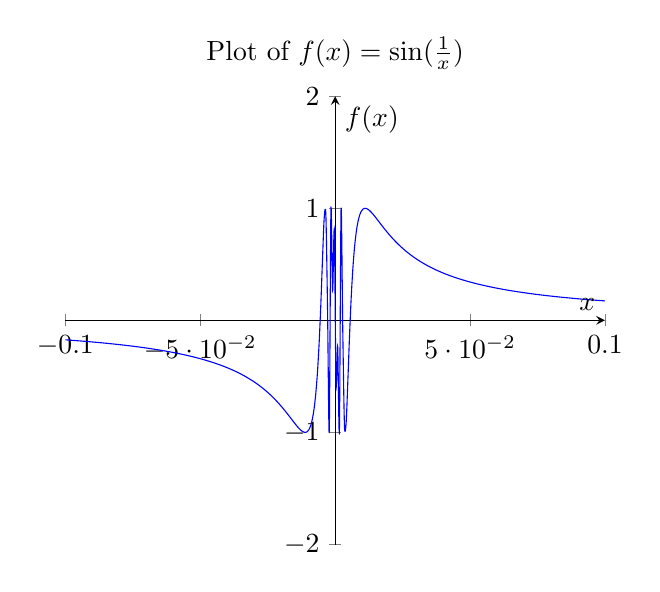
\begin{tikzpicture}
\begin{axis}[
    title={Plot of $f(x) = \sin(\frac{1}{x})$},
    xlabel={$x$},
    ylabel={$f(x)$},
    xmin=-0.1, xmax=0.1,
    ymin=-2, ymax=2,
    samples=800,
    axis lines=middle,
    smooth,
    no markers,
    ytick={-2,-1,0,1,2},
    xtick={-0.1,-0.05,0,0.05,0.1},
    ]
    \addplot+[domain=-0.25:0.25] {sin(1/x)};
\end{axis}
\end{tikzpicture}
\end{figure}

\item The jump function is the simplest form of a discontinuity and has a singularity at the jump.
\begin{figure}
\centering
\begin{tikzpicture}
\begin{axis}[
    title={Plot of the jump function},
    xlabel={$x$},
    ylabel={$f(x)$},
    xmin=-2, xmax=2,
    ymin=-2, ymax=2,
    axis lines=middle,
    smooth,
    no markers,
    ytick={-2,-1,0,1,2},
    xtick={-2,-1,0,1,2},
    ]
    \addplot+[domain=-5:0] {0};
    \addplot+[blue, domain=0:5] {1};
\end{axis}
\end{tikzpicture}
\end{figure}

\item Directly connected to the jump function is the absolute function $f(x) = |x|$. This function does not have any discontinuities, but if we look at the derivative we get once more a jump function that jumps from negative $1$ to positive $1$ at 0. It is important to note that technically this singularity does only belong to the derivative, however, in real-world applications, this is often treated as a singularity of the original function.
\begin{figure}
\centering
\begin{tikzpicture}
\begin{axis}[
    title={Plot of $f(x) = |x|$},
    xlabel={$x$},
    ylabel={$f(x)$},
    xmin=-2, xmax=2,
    ymin=-2, ymax=2,
    axis lines=middle,
    ytick={-2,-1,0,1,2},
    xtick={-2,-1,0,1,2},
    no markers,
    ]
    \addplot+[domain=-2:2]{abs(x)};
\end{axis}
\end{tikzpicture}
\end{figure}

\item For our last example we look at an ideal version of the $\delta$ impulse function. The $\delta$ impulse function is defined as
$\delta(x) = \begin{cases}0 &  x \ne 0\\ \infty & x = 0 \end{cases}$ with an area of $1$. Since both left and right limits are $0$ we could in theory remove the singularity at $x = 0$ by redefining it as $\delta(x) = 0$ but that would destroy the purpose of the $\delta$ function for analyzing the impulse-response of arbitrary systems.
\begin{figure}
\centering
\begin{tikzpicture}
\begin{axis}[
    axis lines=middle,
    xlabel={$x$},
    ylabel={$\delta(x)$},
    ymin=-0.5, ymax=2,
    xmin=-2, xmax=2,
    ytick=\empty,
    xtick=\empty,
    clip=false
    ]

    \draw[blue] (axis cs:0,0) -- (axis cs:0,2);
    \draw[blue] (axis cs:-2,0) -- (axis cs:2,0);
    
\end{axis}
\end{tikzpicture}
\end{figure}
\end{enumerate}

\subsection{Jacobian Matrix}
The second concept we need to introduce is that of the Jacobian Matrix. In the following, we will use simply ``Jacobian'' interchangeably with ``Jacobian Matrix''.
When we work with multivariable functions we often want to predict how changes in inputs affect the output.
Understanding this relationship is crucial for optimizations and modeling real-world phenomena.\\
Functions are called ``linear'' if they satisfy the following two requirements:
\begin{enumerate}
\item $f(\vec{x})+f(\vec{y}) = f(\vec{x} + \vec{y})$
\item $a * f(\vec{x}) = f(a * \vec{x})$
\end{enumerate}
Where $f$ is a function, $\vec{x}$ and $\vec{y}$ are input vectors and $a$ is a scalar.
For transformations that are linear, the relation of input changes to output changes is very straightforward. According to the first requirement any change in the input by $\Delta\vec{x}$ leads to a change of $f(\Delta\vec{x})$ in the output.\\
However, with arbitrary, non-linear functions, the situation becomes more complex. Unlike linear functions, the rate of change in arbitrary functions varies at different points. This variability makes it challenging to predict how a small change in input will affect the output.\\
Here is where the concept of ``local linearity'' comes into play. For any differentiable point on a function, you can approximate its neighborhood by taking the tangential gradient at the point and simply pretending the function was linear.\\

\begin{figure}
\centering
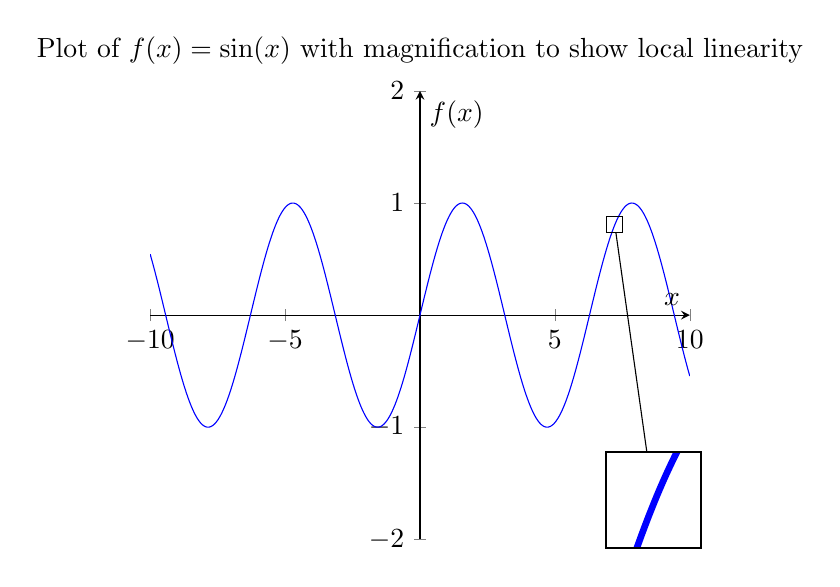
\begin{tikzpicture}[spy using outlines={rectangle, magnification=6, size=0.1\textwidth, connect spies}]
\begin{axis}[
    title={Plot of $f(x) = \sin(x)$ with magnification to show local linearity},
    xlabel={$x$},
    ylabel={$f(x)$},
    xmin=-10, xmax=10,
    ymin=-2, ymax=2,
    axis lines=middle,
    ytick={-2,-1,0,1,2},
    xtick={-10,-5,0,5,10},
    smooth,
    no markers,
    samples=400,
    clip=true,
    ]
    \addplot+[domain=-10:10] {sin(deg(x))};
    \spy [] on (5.9,4) in node [left] at (7,0.5);
\end{axis}
\end{tikzpicture}
\end{figure}

For multivariable functions, we have to take this approach component-wise which in turn means we have to calculate the partial derivative with respect to each component of the input vector. Organizing these derivatives in the form of a matrix leads us to the definition of the Jacobian:\\
The Jacobian Matrix $J$ of a multidimensional function
\begin{center} $f: \mathbb{R}^n \rightarrow \mathbb{R}^m$ \end{center}
is a $m \times n$ matrix that contains each partial derivative of $f$ for one input variable\cite[107]{GdR}.
Each entry is of the form
\begin{center} $J_{ij} = \frac{df_i}{dx_j}$ \end{center}
Unless $f$ is a linear function the resulting Jacobian will still be dependent on the input vector. This means if we want to make predictions about the behavior of the function at a given point $\vec{x}$ we still need to evaluate the Jacobian with respect to $\vec{x}$.

The determinant of the Jacobian Matrix holds significant meaning. To understand this let us first take a step back and recall the meaning of the determinant of an arbitrary square matrix: The determinant is the factor by which the volume of the input vector is changed when compared to the output vector.

\subsection{Example function}
To clarify let us look at the multivariable function $f: \mathbb{R}^3 \rightarrow \mathbb{R}^2$ where f is defined as
$f(x, y, z) = \begin{pmatrix}x^2 + y^2 + z * \sin(x)\\z^2 + z * \sin(y)\end{pmatrix}$\\
To determine the Jacobian we need to find all the partial derivatives:\\
\begin{center} $\frac{d}{dx} f(x, y, z) = \begin{pmatrix}2x + z * \cos(x)\\0\end{pmatrix}$ \end{center}
\begin{center} $\frac{d}{dy} f(x, y, z) = \begin{pmatrix}2y\\z * \cos(y)\end{pmatrix}$ \end{center}
\begin{center} $\frac{d}{dz} f(x, y, z) = \begin{pmatrix}\sin(x)\\2z + \sin(y)\end{pmatrix}$ \end{center}
And the complete Jacobian:\\
\begin{center} $J_f(x, y, z) =
\begin{pmatrix}
  2x + z * \cos(x) & 2y & \sin(x)\\
  0 & z * \cos(y) & 2z + \sin(y)
\end{pmatrix}$\end{center}

Now for an example of a Jacobian Determinant let us consider the following Jacobian:\\
$J(x, y) = \begin{pmatrix}
  -\sin(x) & -\cos(y)\\
  \cos(x) & \sin(y)
\end{pmatrix}$\\
And calculate its determinant:\\
$|J| = -\sin(x) * \sin(y) - (-\cos(y) * \cos(x)) = -\sin(x) * \sin(y) + \cos(y) * -\cos(x)$


\section{Mechanical interpretation}
Many real-world examples can be found in the realm of physics, where many functions contain singularities. At these points certain physical quantities become infinite or undefined, often indicating a breakdown in the normal rules of physics. The most prominent example of this is of course gravitational singularities at the center of black holes. In the following, we will take a specific look at one example from mechanics, a loaded half-plane.

For data and illustrations of this, we will draw from the paper "Differential Equations and the Problem of Singularity of Solutions in Applied Mechanics and Mathematics"\cite{Vasiliev}. This paper challenges traditional approaches to differential equations, especially in scenarios where mathematical solutions face discrepancies with physical observations. For our purposes, however, we will only look at the basic example provided in the paper.

\subsection{Singularities in the simulation of physical stress}
%further explain half-plane
First, let us clarify the term half-plane. A half-plane refers to a concept in mathematics, particularly in geometry and linear algebra. Imagine a two-dimensional plane, like a flat sheet of paper. If you draw a straight line anywhere on this plane, this line divides the plane into two separate regions. Each of these regions is called a half-plane.

For our physical stress experiment, we will take such a half-plane, push a wedge into it, and measure the displacement of points both in the $x$ and $y$ dimensions.

In theory, those displacements can be calculated by the following formulas:
\begin{center}
$u_x(x) = \pm\frac{(1-v)P}{2Eh}$\\
$u_y(x) = -\frac{P}{\pi Eh}(1+v+2\ln{\frac{x}{y_A}})$
\end{center}
To analyze singularities we can ignore the x-Displacement $u_x$ and only focus on the y-Displacement.
Here $E$ and $v$ are material constants, $P$ is the force used to push the wedge, $h$ is the thickness of the plate, and $y_A$ is the $y$ position of the point before displacing it.

\begin{figure}
    \centering
    \includegraphics[width=0.5\textwidth]{images/halfplane_scheme.png}
    \caption{Half-plane with named quantities, taken from \cite{Vasiliev}}
\end{figure}

\begin{figure}
    \centering
    \includegraphics[width=0.5\textwidth]{images/halfplane_photo.png}
    \caption{Photo of the real plate from Vasiliev's\cite{Vasiliev} experiment}
\end{figure}

If we now examine the function for the y-Displacement we notice that due to the use of $\ln(x)$, it has a singularity at $x = 0$ which would translate to an infinitely large displacement at the position of the wedge.
This theoretical outcome conflicts strongly with what can be observed in the real world.

\begin{figure}[H]
    \centering
    \includegraphics[width=0.5\textwidth]{images/displacement_graph.png}
    \caption{Measurments from Vasiliev's experiment compared to theoretical results, the dashed curve is the calculated result, the points are the measurements from the experiment and the solid line is the curve interpolated from the sample points}
\end{figure}


\section{Interpretation in Robotics}
Discrepancies between predictions and reality like the one shown in the last chapter may be intuitive to spot for a human, after all, we know from experience that pressure against objects does not lead to infinite displacements. But they can cause real havoc when automated systems encounter them without being equipped to deal with these corner cases. A prime example of this is the problems that arise in robotics from singularities in their control systems.

\subsection{Kinematics basics}
Kinematics is a branch of mechanics that focuses on the motion of objects without considering the forces that cause this motion. It deals with parameters like velocity, acceleration, displacement, and time, providing a mathematical framework to describe an object's position and motion in space. In robotics, kinematics is crucial for designing and controlling robot movements. It is divided into two main types: forward kinematics, which predicts the position of the end-effector given joint angles, and inverse kinematics, which calculates the required joint angles to achieve a desired end-effector position. Understanding kinematics is fundamental for accurately programming and operating robotic systems.

Let us study these two concepts in a bit more detail.
For these explanations, we consider a robot manipulator, which is a series of joints. The end of this chain is called the end-effector. This end-effector might be something like a gripper, a tool, or a foot in a real robot.

\subsection{Forward Kinematics}
Forward kinematics is a fundamental concept in robotics that deals with the computation of the position and orientation of a robot's end effector based on the known joint parameters, such as angles for rotational joints or distances for prismatic joints. Every robot manipulator consists of a series of joints, each joint can be described by a transformation matrix that takes coordinates from our reference plane to the rotated or translated point.

\subsection{Inverse Kinematics}
In most cases, we do not know the joint configurations but we do know the desired position of the end-effector. In these cases, we must turn towards inverse kinematics to find the required joint configurations. There are multiple ways to solve this problem, algebraic, geometric, and several numerical solutions do exist. We will only consider an iterative Jacobian-based approach\cite[94]{GdR} as that gives the best insight into singularities.

For this approach, we need to recall two things and put them together. First, the Jacobian Matrix is the matrix of all partial derivatives of a multivariable function. Second, thanks to forward kinematics we have a function that takes all joint angles and maps them to the position of the end-effector. Now if we put these two together we get a Jacobian that maps the derivative of joint angles to the derivative of the end-effector position. What makes this interesting to us is that the derivative of angles are angle velocities and the derivative of a position is just a velocity.

In other words, the Jacobian Matrix of a robot manipulator is the matrix that maps its joint velocities (either angles in a rotational joint or distances in a translational joint) to the velocity of the end-effector\cite[29]{HandbookOfRobotics}.

Armed with this knowledge let us go through the inverse kinematics approach step by step\cite[95]{GdR}:
\begin{enumerate}
    \item Obtain changes in joint configuration $\Delta\vec{x}$
    \item Calculate the wanted change in end-effector position by subtracting the current end-effector position from the wanted end-effector position
    \item Apply the result of step 2 to the inverse Jacobian to get needed changes in joint angles
    \item Use the resulting joint velocities to modify the robots state
    \item After calculating  the Jacobi-matrix is updated
    \item Repeat
\end{enumerate}

This approach however suffers from one problem that can cause it to fail. In step 3 we assume that the inverse of the Jacobian exists, but this is not necessarily the case.

For square matrices, the invertibility of a matrix can be checked by calculating its determinant.
If $|M| = 0$ with $M$ being the matrix, then $M$ is not invertible\cite{MatheKagga}.
If this is the case, $M$ is called singular.

For rotational joints, this is the case if two joints are aligned at $0$\textdegree \ or $180$\textdegree \ because the linearized gradients of the joints are exactly perpendicular to the link\cite[5]{PatrickVonwirth}. Any motion in the direction of the link would have multiple equivalent paths, which leads us to why this phenomenon is called singularity. The usage of the term ``Singularity'' in robotics arises from the expression of two things being ``singular'' as in being one.
The Springer Handbook of Robotics defines Singularities in Robotics as follows ``regions where two or
more joints may become aligned or nearly aligned''\cite[78]{HandbookOfRobotics}.
In these points, the robot experiences a loss of one degree of freedom, which results in the robot stopping moving or moving in an unexpected manner.

Now let's apply these principles to an example and study the resulting singularities.

\subsection{Example Robot: Planar, Two-Segment Arm}
To illustrate this behavior on a real robot we study the following two-dimensional robot arm:

\begin{figure}[H]
    \centering
    \includegraphics[width=0.5\textwidth]{images/robot_arm.png}
    \caption{Planar robot arm}
    \label{fig:robot_arm}
\end{figure}

To analyze this robot let us determine the forward kinematic equations.\\
$\begin{pmatrix}
  x \\ y
\end{pmatrix} = \begin{pmatrix}
  l_1 * \cos(\alpha) + l_2 * \cos(\alpha + \beta)\\
  l_1 * \sin(\alpha) + l_2 * \sin(\alpha + \beta)
\end{pmatrix}$\\
Where $(x, y)$ is the position of the end-effector, $l_1$, $l_2$, $\alpha$ and $\beta$ are as shown in \autoref{fig:robot_arm}.\\
As shown in the mathematical foundations chapter, to find the Jacobian we have to take the partial derivatives with respect to $\alpha$ and $\beta$:\\
$J(\alpha, \beta) = \begin{pmatrix}
  -l_1 \sin(\alpha) - l_2 \sin(\alpha + \beta) & -l_2 \sin(\alpha + \beta)\\
  l_1 \cos(\alpha) + l_2 \cos(\alpha + \beta) & l_2 \cos(\alpha + \beta)
\end{pmatrix}$\\
To search for singularities we search for positions where $|J| = 0$.\\
$|J| = (-l_1 \sin(\alpha) - l_2 \sin(\alpha + \beta)) * l_2 \cos(\alpha + \beta) + l_2 \sin(\alpha + \beta) * l_1 \cos(\alpha) + l_2 \cos(\alpha + \beta)$\\
When $\beta$ is $0$\textdegree \ or $180$\textdegree \ the determinant becomes 0 indicating a singularity.

To get a visual grasp on this let us look at \autoref{fig:robot_arm_singularity}, $\beta$ is $0$\textdegree \ here and as we can see the linearized gradients of the velocity are perpendicular to the rest of the robot arm, resulting in the loss of one degree of freedom.

\begin{figure}[H]
    \centering
    \includegraphics[width=0.45\textwidth]{images/robot_arm_singularity.png}
    \caption{Planar robot arm in singular position}
    \label{fig:robot_arm_singularity}
\end{figure}


\section{Conclusion}
In this seminar paper, we have embarked on an extensive exploration of singularities, focusing on their mathematical foundations and mechanical interpretations, particularly in the realm of robotics. Through a journey that spanned from the intricacies of mathematical singularities to practical robotic applications, we've observed how singularities influence both theoretical and real-world scenarios.

Key Insights and Implications:
\begin{itemize}
    \item Mathematical Foundations: We began by dissecting the mathematical aspects of singularities, understanding their definitions and implications in various functions and equations. By categorizing singularities we have gained an understanding of important characteristics that help us in the following real-world applications of singularities.
    \item Application to mechanics: As one of these real-world applications we looked at a manifestation of singularities in mechanical stress on objects. Where the predictions from theory differed from measurments taken in an experiment.
    \item Robotic Singularities: We then transitioned into the realm of robotics, where we applied these concepts to analyze singular configurations in robotic systems, emphasizing kinematics. As an illustration of this, we took a closer look at a simple planar arm robot, exploring how singularities can manifest in mechanical systems, impacting their functionality and control.
\end{itemize}
Singularities, both as a mathematical concept and a practical challenge in robotics, offer a rich field for exploration and innovation. This paper has aimed to bridge the gap between abstract theory and tangible application, shedding light on a topic that is as challenging as it is fascinating.


\bibliographystyle{IEEEtran}
\bibliography{agrosy}


\end{document}

